\documentclass[a4paper,man,natbib]{apa6}

%%%%%%%%%%%%%%%%%%%%%%%%%%
% Thesis-specific settings
%%%%%%%%%%%%%%%%%%%%%%%%%%

%%%%%%%%%%%%%%%%
% Theme settings
%%%%%%%%%%%%%%%%

\usepackage{times}

\usepackage{graphicx}
\usepackage{epstopdf}

%PURE's ADD
\usepackage{epsfig}
\usepackage{subfigure}
%\usepackage{indentfirst}
\usepackage{url}
\usepackage{array}
%END PURE's ADD

\title{Spatial Features in Classification of Points-of-Interests}
\shorttitle{Spatial Features in Classification of POIs}
\fourauthors{Youer Pu}{Kaiqi Zhao}{Gao Cong}{Kenny Q. Zhu}
\fouraffiliations{Department of Computer Science \& Engineering\\ Shanghai Jiao Tong University\\ Shanghai, China}{School of Computer Engineering\\ Nanyang Technological University\\ Singapore}{School of Computer Engineering \\ Nanyang Technological University\\ Singapore}{Department of Computer Science \& Engineering\\ Shanghai Jiao Tong University\\ Shanghai, China}


%\usepackage{apalike}
%\bibliographystyle{apalike}

\usepackage{apacite}
\bibliographystyle{apacite}


\usepackage{amsmath,amssymb,amsthm}

\usepackage{algpseudocode}

\newcommand{\KQ}[1]{\textcolor{red}{[KQ: #1]}}
\usepackage[normalem]{ulem}
\usepackage{listings}
\usepackage{color}

%%%%%%%%%%%%%%%%%%%%%%
% Document starts here
%%%%%%%%%%%%%%%%%%%%%%

\abstract{
The category (or type) of a point-of-interest (POI) is 
important for location based services (LBS). Popular mapping services try to
include POI type information or allow map users to tag POIs from a 
predefined set of categories, but these tags can be inaccurate and far 
from complete.
The classification of POIs have been studied in the context of location-based
social network and the models developed there 
are largely based on user visiting behaviors.
This paper explores another aspect of POIs: the geographical 
location of a POI, and studies how spatial features influence the results of
POI classification. 
We find that different spatial features work well for different categories, 
and a best feature combination exists for each category. 
We show that while each feature individually benefits the classification, 
the best combination provides significant improvements over user behavior 
features alone. What's more, spatial features are robust to noise and sparse
data.
}

\begin{document}

%\pagenumbering{gobble} % disable page numbering

\maketitle


\section{Introduction}
\label{intro}
As smart phones penetrate in the world's populations,
applications are increasingly
tracking user locations and offering services based on where the users are or
where they frequently go. Pure latitudes and longitudes provided by GPS
are not useful until they are correlated to specific locations on a map which
carry semantics. These meaningful locations, which are known as
point-of-interests, or POIs, include transport hubs, restaurants,
schools, scenery spots, office buildings, etc. POIs serve as the
basic components in location-based services (LBS) for exploration and 
recommendation.

Ordinary maps provide the names of the POIs only. But not all names are
indicative to the type or category of the POIs, which is extremely useful
information for determining the semantics of the location.
In addition to providing semantics for each POI, categories
naturally group together POIs which are similar to each other
by some common characteristics.
Online mapping services such as Google Map have started to add
category information for
POIs as tags, often manually labeled by the map provider or the user community.
However, such category tags are far from being complete.
For example, Figure \ref{fig:vivo} shows an area in
central Singapore on Google Map.
Some of the POIs are labeled with categories such as ``Food'',
``Shops'' and ``Banks'' (indicated by graphical icons).
Others, such as ``Best Denki'', does not have a label.
Without prior knowledge, it would be hard to know that ``Best Denki''
in Singapore is actually an electronics retailer.

Unfortunately, many of category labels are missing in today's maps
or location-based social networks (LBSN).
According to the survey from Ye et al. \cite{yemao}, about 30\% POIs in
Whrrl (which is a well-known LBSN) lack category information,
which is a substantial loss of information for the map.

In this paper, we aim to automatically classify POIs on the map of a LBSN
into different categories. In this paper we employ a global classification
hierarchy from Foursquare, showed in Table \ref{tab:Categories},
as the standard categories. This hierarchy provides categories in different
granularity, designed for both general needs and specific interests.
For example, ``Best Denki'' will be first classified as ``Shop \& Service'',
which is a first level category identifying its general purpose.
It can be further classified as ``Electronics Store'',
which is a second level category with more details.
Most of the existing proposals consider only
the first level, general categories. However, 
a POI may belong to more than one category.
For example, many bars offer dinner service as well,
which qualifies them as both ``Food'' and ``Nightlife''.
Moreover, according to our experiments,
spatial features also contribute to better performances for
second level categories. 
A standard category hierarchy works better than
ad hoc labels provided by users. For example, ad hoc labels such as
``restaurant'', ``buffet'', ``cafe'' , ``burger joint'', ``pizza place'',
all belong to the standard ``Food'' category, which avoids confusion.

\begin{figure}[ht]
  \epsfig{file=VenueGraph/vivocityrec.eps,width=\columnwidth}
\caption{Vivocity, Singapore (from Google map)}
\label{fig:vivo}       % Give a unique label
\end{figure}

\begin{table}
\caption{1st Level Category and Examples of 2rd Level Category}
\label{tab:Categories}
\begin{tabular}{p{4cm}|p{10cm}}
\hline

1st Level Category&	Examples of 2nd Level Category\\
\hline
Arts \& Entertainment&	Aquarium, Art Gallery, Casino, Concert Hall, Movie Theater, Museum, Stadium, Theme Park, Zoo\\
\hline
College \& University&	College Academic Building, College Library, College Residence Hall, College Stadium, Law School, Medical School\\
\hline
Food&	American Restaurant, Buffet, Cafeteria, Chinese Restaurant, Ice Cream Shop, Pizza Place, Tea Room, Wings Joint\\
\hline
Nightlife Spot&	Beach Bar, Beer Garden, Lounge, Karaoke Bar, Sake Bar, Sports Bar\\
\hline
Outdoors \& Recreation&	Athletics \& Sports, Beach, Castle, Farm, Fishing Spot, Forest, National Park, Palace, Ski Area, Vineyard\\
\hline
Professional \& Other Places&	Animal Shelter, Factory, Government Building, Medical Center, Non-Profit, Office, School, Spiritual Center\\
\hline
Residence&	Home (private), Residential Building (Apartment / Condo), Trailer Park\\
\hline
Shop \& Service&	Bank, Bookstore, Car Wash, Clothing Store, Electronics Store, Gym / Fitness Center, Outlet Store, Pet Service, Spa\\
\hline
Travel \& Transport&	Airport, Boat or Ferry, Bus Stop, Hotel, Subway, Taxi, Train Station\\
\hline
\end{tabular}
\end{table}

LBSNs carry not only
names, geographical coordinates, but also users' check-in records.
We formulate the problem as a supervised multi-label classification problem,
since some of the POIs are labeled with categories by users and some are not.
Then we solve it in a typical classification setting by extracting features
from raw data and use them as input for a classifier, which produces the
category labels.

The most intuitive features of POIs would be word features extracted
from the names. Besides that, some work, e.g., Ye et al. \cite{yemao},
has focused on the user check-in activities.
They use features based on statistics of user behaviors,
including population features (e.g., the total number of check-ins at a POI)
and temporal features (e.g., 24-hour distribution of check-in time).
These features turn out to be effective, and are considered BASE features
in this paper as well.

However, even though user behavior is an effective feature,
formulating users' interest profile purely on check-in records 
for the POI classification problem has some serious limitations.
The reasons are as follows.
First, normal users' check-in frequency is insufficient to make a
reasonable profile of a user's visit preferences,
and there may be very active users who check in a lot but may not check in
to all uncategorized POIs
Second, unlike movies or music, for which user behaviors depend almost
entirely on user interest, the check-in behavior of an individual user
is only partly influenced by user's interest,
and probably more affected by her life style, e.g., place of work, 
usual shopping places, usual restaurants, etc. These are strongly correlated 
with the active geographical area of the user, such as where they live or work.
Without differentiating user's real preference and their normal life,
connections between the places introduced by individual users would not
be convincing for POI classification. In other words, POI categories are not
so much distinguished by who visit them, but by {\em how} they are visited,
e.g., time, date and frequency, etc.
That explains why statistics over large number of users,
such as 24-hour check-in distribution and 7-day check-in distribution turn
out to be more effective in classification according to Ye et al.'s work \cite{yemao}.

In our work, we discover that the spatial aspects of POIs which
has not been considered in the past can potentially complement
the name and user behavior features and thus improve the accuracy of POI
classification.
Although POIs which are close to each other are not necessarily from the same
category, the location of a POI is almost never random
but a deliberate choice when it was established, and it is
heavily influenced by the category of the POI and the neighbors around it.
The following example illustrates why spatial features are useful
when there is insufficient user check-in data and little clue from the
name of the POI. Figure \ref{fig:EgCasa} shows a POI
called ``Casa Bom Vento'' in Singapore. The name is not in English,
which means word features are not very useful.
The place is also not very popular, and has only attracted one check-in 
record in the past, which means user behaviors cannot help.
Fortunately, the POI is surrounded by many restaurants, which increases
the odds that it belongs to the ``Food'' category.
POIs in the same categories are gathering together as shown
in Figure \ref{fig:EgCasa}, and tend to have
similar neighborhood. For example, restaurants and shopping malls are
often near each other as shown in Figure \ref{fig:vivo}. 
Moreover, POIs in category other than ``Food'' may have 
other surroundings. For example, ski parks are often alone by themselves 
as shown in Figure \ref{fig:skipark}.

\begin{figure}[ht]
\begin{minipage}[ht]{0.51\linewidth}
\centering
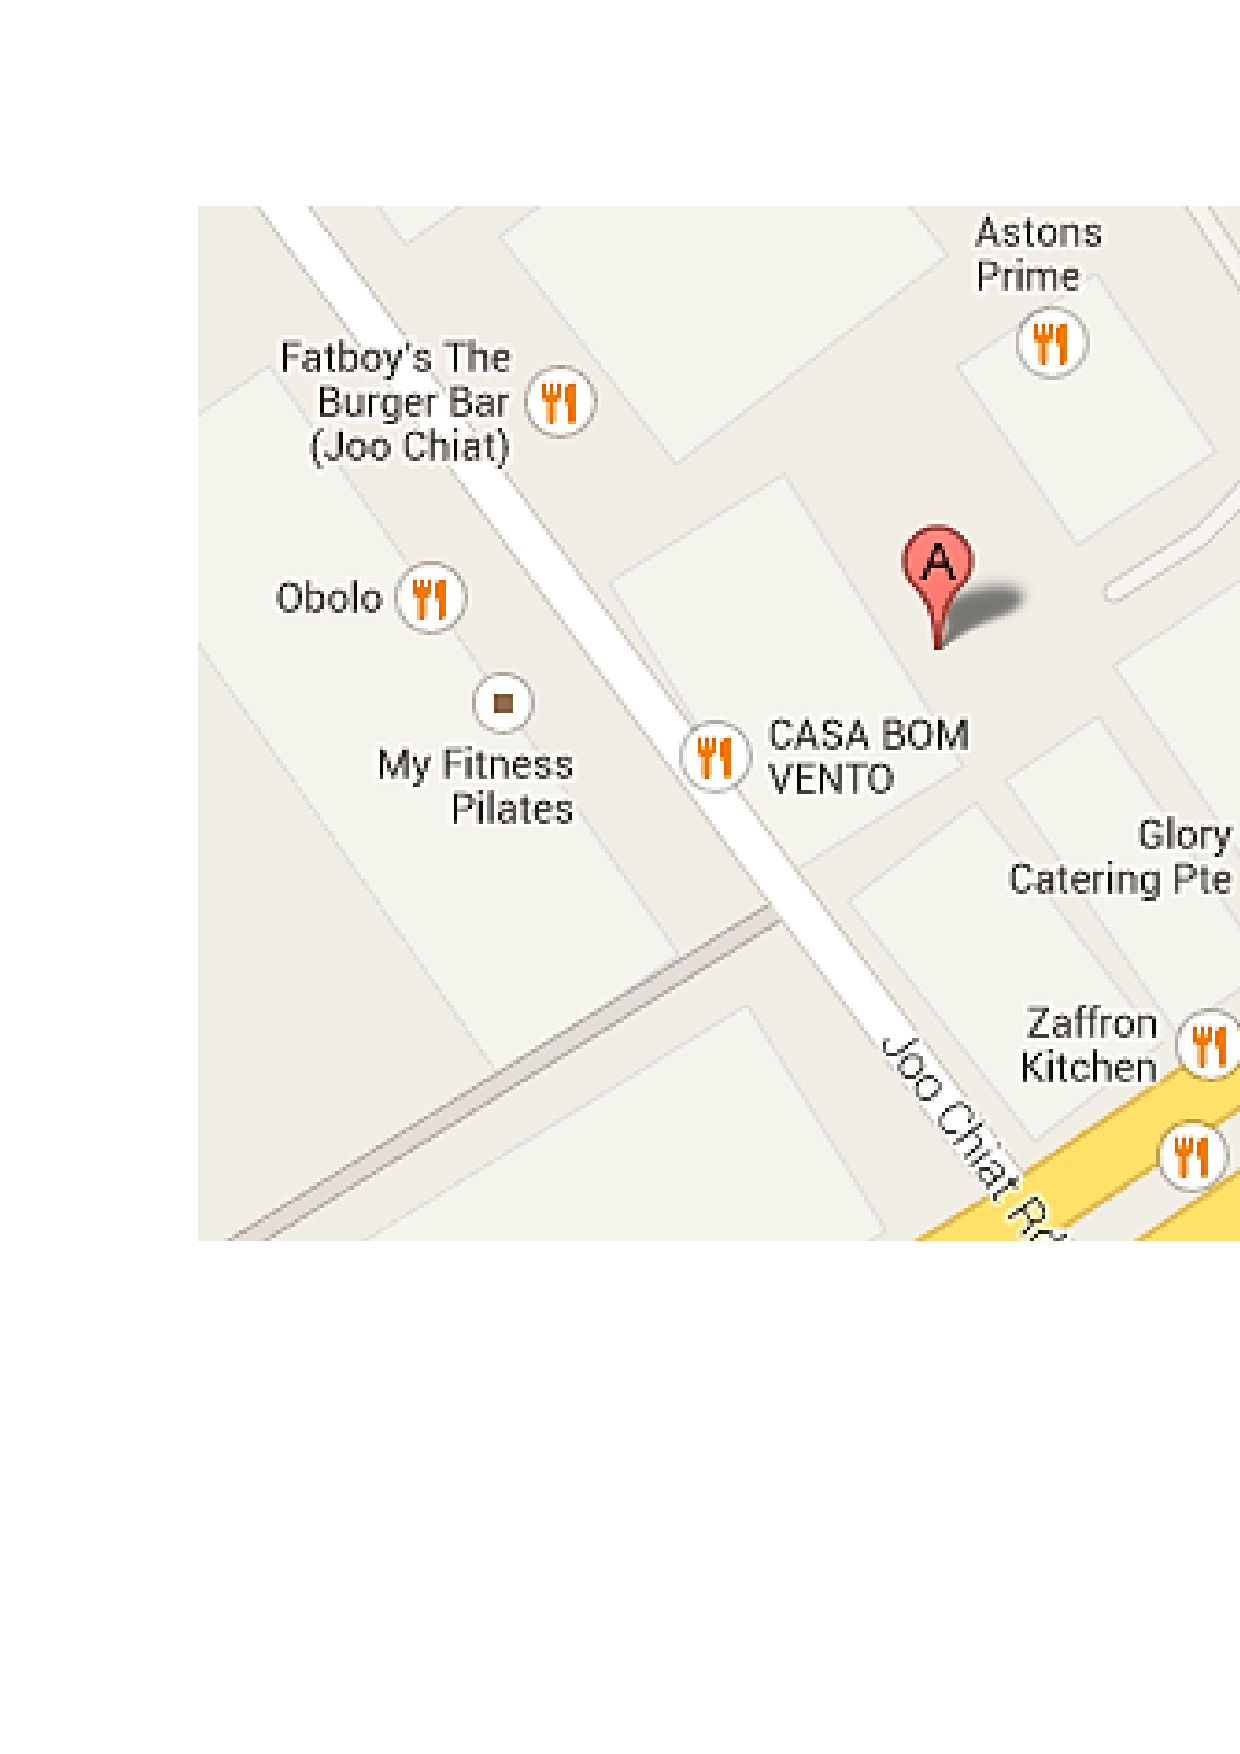
\includegraphics[width=\columnwidth]{VenueGraph/CasaBomVento.PNG}
\caption{Casa Bom Vento, Singapore (from Google map)}
\label{fig:EgCasa}
\end{minipage}
\hspace{0.5cm}
\begin{minipage}[ht]{0.49\linewidth}
\centering
\includegraphics[width=\columnwidth]{VenueGraph/skipark.eps}
\caption{Catfish Bay Water Ski Park, United States (from Google map)}
\label{fig:skipark}
\end{minipage}
\end{figure}

In this paper, we focus on exploring spatial features for POI classification.
We propose a number of spatial features and ways to extract them.
Then, we briefly introduce other features,
including NAME and BASE.
Finally, we show how spatial features complement
the name features and check-in statistics features
to further improve the classification results.
We also conduct experiments on second level classification,
and show stable advantage over the baseline.

Some of the proposed spatial features focus on locations;
while others compute the user behavior statistics of
POIs within certain distance.
These features show different strength and capabilities in identifying
different categories. We will discuss such differences and fine-tune
the best combination of features for each category.
This paper makes two main contributions:
\begin{itemize}
\item We exploit relative positioning among POIs in combination
with check-in records of users, and
analyze several spatial characteristics in different kinds of POIs;
\item We show spatial features are individually distinctive and effective,
and we manage to produce the best feature combination for each category.
The result outperforms the baseline method using only name features and
user behavior features on real data from Foursquare.
\end{itemize}

\section{Spatial Features}
\label{chp:spatial}
Considering only one POI's location, it can be as simple as a pair of
longitude and latitude.
However, with relative position with other POIs, more information emerges.
Such information is closely related to the POI's functional characteristics,
which indicate their categories. POIs with different categories show different
characteristics on many statistics related to spatial aspects as explained
below, and thus different features work well on different
categories. In the following, we analyze different kinds of spatial features
on a segment of the New York data crawled from Foursquare.
We consider only the first level categories for simplicity,
because the same features can be applied to the second level categories
(shown in experiments).

\subsection{Neighborhood Category Distribution}

We observe that POIs related to each other often appear in the same zone.
For example, a shopping center has shops and restaurants; a financial center
has banks and office buildings; a college town has colleges, museums,
and observatories. Neighborhood shows functionality of an area and thus
provides a prior probability of the category a POI may belong to. In addition,
since different categories show great differences in the composition of 
their neighborhoods, neighbourhood profile is also good at 
differentiating POIs in different categories.

As shown in Figure \ref{fig:NoPOI}, according to our analysis on POIs in 
New York from Foursquare data, around 30\% of ``Outdoors \& Recreation'' 
have no other POIs near them within 100 meters, 
indicating their ``isolation''; while most of ``Food'' have
other POIs near them, indicating a symbiotic relationship of ``Food'' with other
interesting spot. The reason is that people often visit a restaurant when 
they are on the way to or leaving some POIs like shops, cinemas, etc. 
On the contrary, POIs in
``Outdoors \& Recreation'' are usually built in a
large open space, far from other attractions.
From the figure we can also
see that ``Nightlife Spot'', ``Shop \& Service'' are often close to
other POIs, too, which coincides with the common sense.

Not only the ``crowding'' within a POI's neighborhood differs 
from one category to another,
the category distribution of the neighborhood also differs from one another.
First, we notice that there exists some extreme cases in the category
distribution, such as ``Food'' is everywhere while there's very few ``colleges''
near any POIs in the city. However, difference still stands out between 
categories.  As shown in the Figure \ref{fig:ShopProf} we can see 
there are more food and shops
around ``Shop \& Service'', but there are more ``College \& University'',
``Professional \& Other Places'' near ``College \& University''.

Therefore, we introduce NB\_m feature to describe the category distributions
within certain distance around the POI. The NB\_m feature is defined as:
for a POI $i$, the category distribution of all the POIs
within $i$'s m meters and the number of POIs within m meters.

\begin{figure}
  \centering
  \begin{minipage}[b]{.4\linewidth}
    \centering
    \includegraphics[width=\columnwidth]{plot/No_other_POI_within_100m.eps}
  \end{minipage}%
  %\hspace{-0.75cm}
  \begin{minipage}[b]{.6\linewidth}
    \centering
    %\includegraphics[width=\columnwidth]{plot/Shop_and_Service_and_Professional_and_Other_Places_neighbor_within_100m.eps}
    \includegraphics[width=\columnwidth]{plot/ColorMap/Shop_and_Service_and_Professional_and_Other_Places_neighbor_within_100m.eps}
  \end{minipage}\\%[-10pt]

  \begin{minipage}[t]{.4\linewidth}
    \caption{No other POIs within 100m}
    \label{fig:NoPOI}
  \end{minipage}%
  \hspace{0.3cm}
  \begin{minipage}[t]{.55\linewidth}
    %\caption{Shop \& Service's and Professional \& Other Places 's neighbor within 100m}
    \caption{Nearby Category Distribution within 100 Meters (ytics) for Different Categories'(xtics)}
    \label{fig:ShopProf}
  \end{minipage}%
\end{figure}

\subsection{ The Nearest K POIs}
Apart from neighborhood functionality, we find the nearest $k$ POIs'
category to be another feature that can compensate the NB\_m feature.
It is because the NB\_m feature represents the general
functionality in a big area, but there are often 
concentrations of the same type of POIs in specific spots. 
As shown in Figure \ref{fig:foodcollege},
``Food'' and ``College \& University'' show typical intention
aggregating on some spots. For ``College \& University'', whether
they are located in urban or suburban areas, 
the college buildings are always close to each other. 
As for ``Food'', we can see the trend very often
in our life: there might be a street of local snack, or a part of
business zone full of restaurants. Besides that, other than similar POIs
aggregating together, some categories instinctively near together.
For example, ``Nightlife Spot'' are often mixed with ``Food'',
which is another typical characteristic for both ``Nightlife Spot'' 
and ``Food''.

It seems that the nearest $k$ POIs feature is a part of POI's neighborhood 
feature.  However, focusing on the nearest POIs gives extra information 
on the particular location that the POI is in.
For example, although the neighborhood mainly consists of office buildings,
if the target POI lies in a part of the region that is full of restaurants,
it is more possible that the POI belongs to ``Food''.
In other words, POI's neighborhood considers a neighborhood based on
the absolute distance, which not only represents the neighborhood's attributes,
but also tells how busy that region is.
The nearest $k$ POIs feature is a relative neighborhood that considers
only the nearest $k$ POIs, no matter how far away or how close they are 
from each other. In fact, the two kinds of feature do show
big differences in the experiment and we cannot replace one with another.

We use N\_k to abbreviate the nearest $k$ POIs' category distribution.
The N\_k feature is defined as: for a POI $i$, the category distribution 
of nearest $k$ POIs within 1km to $i$.

\begin{figure}[ht]
\centering
%\includegraphics[width=0.7\columnwidth]{plot/Food_and_College_1-Nearest_POI_category_distribution.eps}
\includegraphics[width=0.8\columnwidth]{plot/ColorMap/Food_and_College_1-Nearest_POI_category_distribution.eps}
\caption{The Nearest POI's Category Distribution for Different Categories}
\label{fig:foodcollege}
\end{figure}

\subsection{Distance to Category}
\label{sec:lcd}
The NB\_m and N\_k feature are insufficient for identifying the category of a
POI in some cases. For example, if a POI is located close to a 
lot of restaurants,
then the POI is supposed to be in category ``Food'' according to the NB\_m and N\_k features.
However, if the POI is far from ``Shop \& Services''
and ``Art \& Entertainments'', then the
POI is probably not a restaurant but a residence.
Due to this fact, we also examine the influence of category
distance, which is the distance from the target POI to
the nearest POI in each category.
Specifically, we first examine average distance from any category to
the nearest ``Travel and Transport'' to see which categories are often
near transportation. We show the distances in Table \ref{tab:DisToTravel},
and we find that ``Professional \& Other Places'' is the 
nearest to transportation, which is reasonable since these places usually
have large number of employees who travels between home and work daily.

\begin{table}[ht]
\centering
%\small
% table caption is above the table
\caption{Different Categories' Average Distance to Nearest ``Travel and Transport''}
\label{tab:DisToTravel}       % Give a unique label
% For LaTeX tables use
\begin{tabular}{llll}
\hline\noalign{\smallskip}
Category & Distance(m) &Category & Distance(m) \\
\noalign{\smallskip}\hline\noalign{\smallskip}
Professional \& Other Places  &    \textbf{210.851} &   College \& University  &    275.849   \\
Nightlife Spot  &   227.3833 &Residence  &   308.1981 \\
Shop \& Service  &   227.5524 &Travel \& Transport  & 9788.035\\
Arts \& Entertainment  &   230.5648 &  Outdoors \& Recreation & 12272.19\\
 Food  &   237.8074 & & \\
\noalign{\smallskip}\hline
\end{tabular}
\end{table}

Then, we examine the distance of each category to all other categories in Figure \ref{fig:LogCD}.
From the figure, we observe that ``Outdoor \& Recreation'' is far from all categories,
while ``Food'' is near to all.
This fact goes in line with our analysis in Figure \ref{fig:NoPOI} that
there are very few POIs near ``Outdoor'', but ``Food'' can be found everywhere.

Formally, we define the category distance feature ($CD$) for a POI $i$ 
and a category $c$ as:
\begin{equation}
CD_{i,c}= min_{j \in c} distance(i,j).
\end{equation}

The linear definition of category distance is straightforward but deviates from
the reality. POIs in 100km from the target POI and those in 200km
have not much difference for identifying the target POI's category because
both of them are too \emph{far}. In contrast, the classifier should 
be sensitive to the difference between two short distances. 
Therefore, we propose two
variations to $CD$, i.e., $LCD1, LCD2$ as follows:
\begin{align}
LCD1_{i,c} &= \log{(1+CD_{i,c})},\\
LCD2_{i,c} &= \log{(1+\log{(1+CD_{i,c})})}.
\end{align}

\begin{figure}[ht]
\centering
\includegraphics[width=0.8\columnwidth]{plot/ColorMap/Color_CategoryDis.eps}
%\caption{Log(Avg(Category Distance))}
\caption{Average Log-distance between Categories (Darker color 
indicates larger distance)}
\label{fig:LogCD}
\end{figure}

\subsection{Region Comparison}
Region Comparison feature aims at comparing the target POI with 
other POIs within the same region on the user behaviors. 
The motivation is that some categories
may often be ``destinations'' of a user's travel activity, 
such as ``Art \& Entertainment'', while other categories may often 
be on the way to the destination, such as ``Food''.
We assume that the places which are more popular (according to users 
and check-ins) than other places nearby, is more likely to be a destination. 
To make use of the user check-in information, we consider both the 
number of check-ins and the number of unique users. We compare the check-ins 
and unique users of the target POI to the POIs within a distance of $m$,
and compute the average difference of check-ins and unique users as the
region comparison feature for the POI. The region comparison feature for total
check-ins ($RC\_T\_m(i,c)$) and for unique users ($RC\_U\_m(i,c)$) are 
computed as follows:
\begin{equation}
RC\_T\_m(i,c) = Avg_{j \in c, distance(i,j)<m} \#Checkin(j) - \#Checkin(i) 
\label{eq:rct}
\end{equation}
\begin{equation}
RC\_U\_m(i,c) = Avg_{j \in c, distance(i,j)<m} \#UniqueUser(j) - \#UniqueUser(i)
\label{eq:rcu}
\end{equation}

Figure \ref{fig:RC} shows the average region comparison feature of 
total check-ins for the five categories of POIs.
The score below 0 means that people check in more times at target POI than the POIs near it.
Intuitively, ``Art \& Entertainment'' is more of a ``destination'', because
people come in to watch a show, or see an exhibition. 
``Outdoor \& Recreation'' is more of a ``destination'', too,
since people plan in advance to have a weekend with children on a beach, 
or have a day off to fishing spot. ``Food'' is a ``on the way'' category 
both by intuition and statistics. People grab something to eat all the time: 
after a walk or before a movie. Interestingly, we
find that ``Shop \& Service'' shows the character of a ``by the way'', too.
It seems interesting shops are growing in numbers, and consequently 
people are attracted into a shop though not intended. In contrast, 
nightlife spots are more of destinations, because they 
are usually the last places people may visit in a day. 

\begin{figure}[ht]
% Use the relevant command to insert your figure file.
% For example, with the graphicx package use
  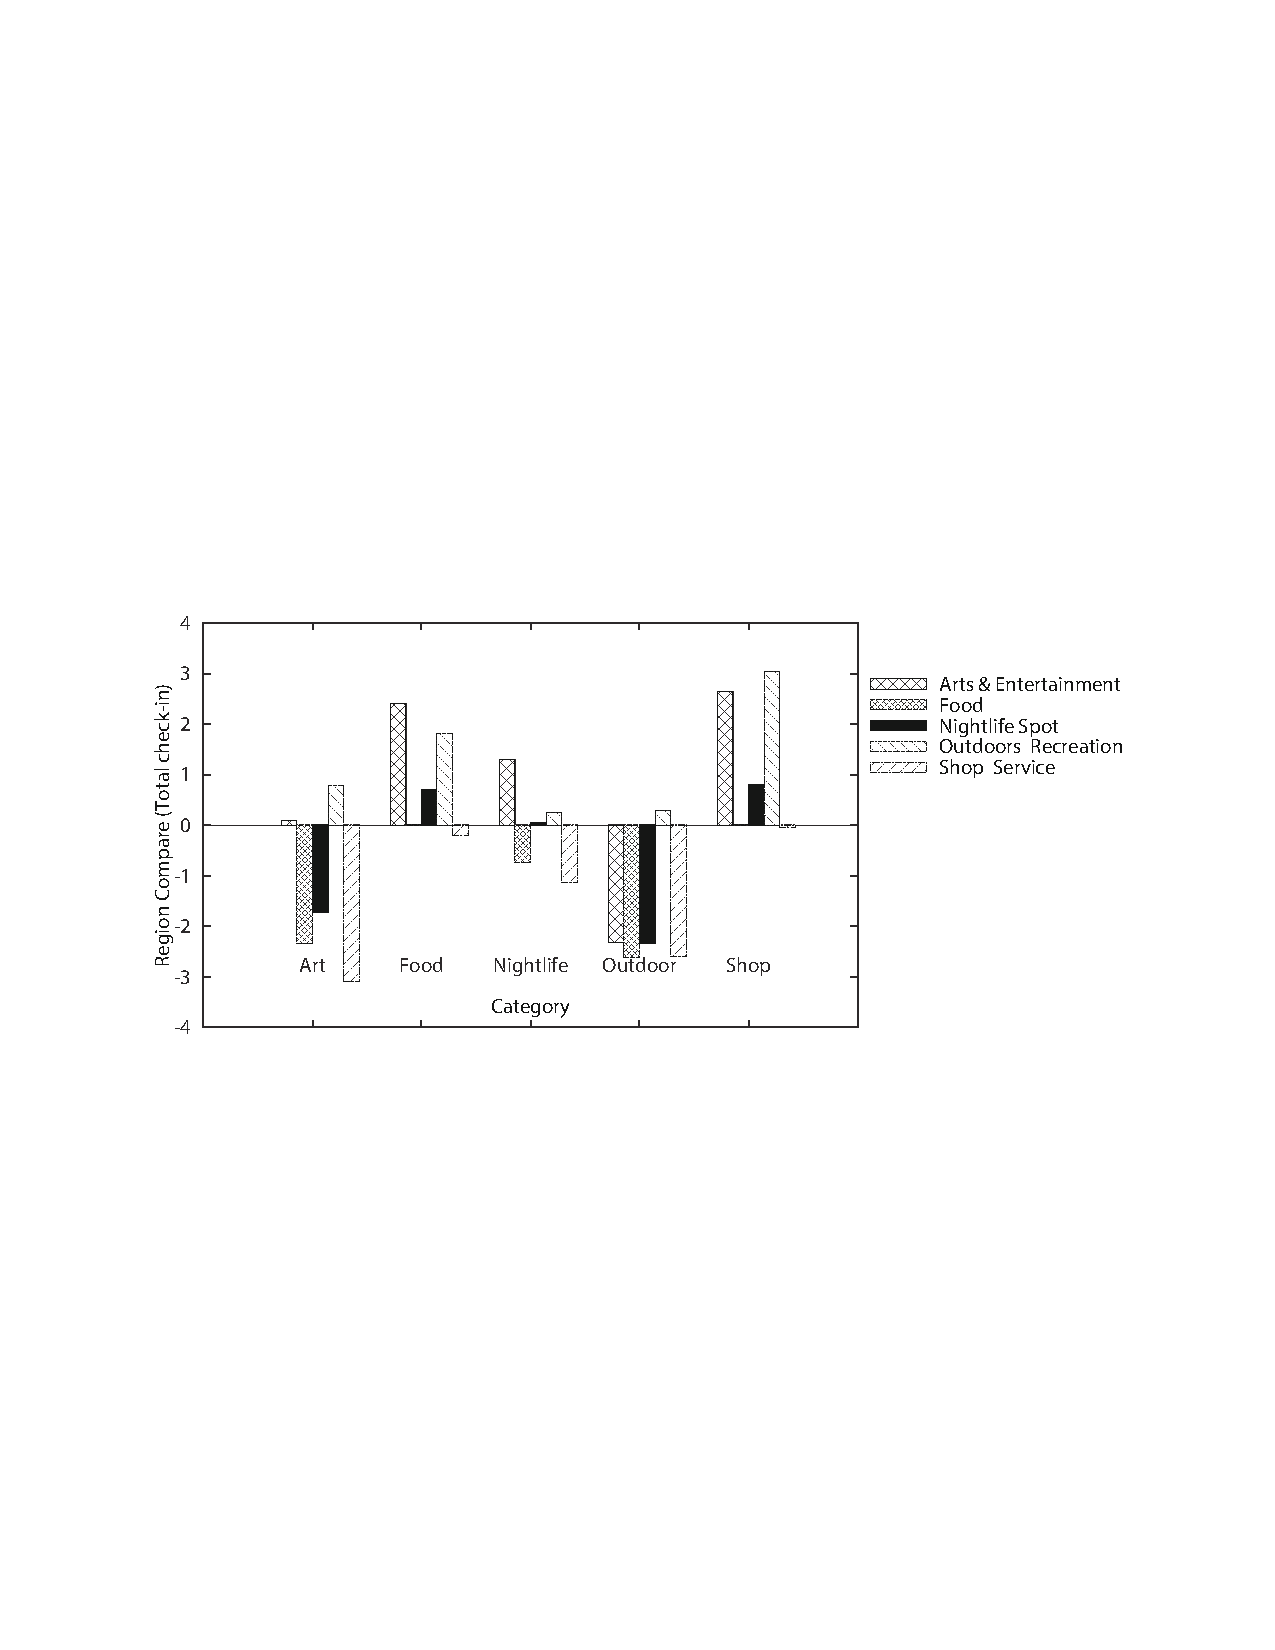
\epsfig{file=plot/RegionCompare.pdf,width=\columnwidth}
% figure caption is below the figure
\caption{Region Compare for Total Check-ins (Score below 0 indicates more check-ins than other categories within the same region)}
\label{fig:RC}       % Give a unique label
\end{figure}

\section{Other Features}
\label{chp:others}
\subsection{NAME Features}
The most direct way to discover the category of a POI is looking at its name.
%Similar with human guessing the category of a POI, the first intuition we get from a POI is its name.
For example, when we see a POI named ``Mouth Restaurant'', we would easily figure out that it belongs to ``Food''.
%Given the fact that words appear in POIs' names are far more less than in vocabulary,
We build the NAME feature in a straightforward way. We break POIs' names 
into words, then we collect all the words and filter out those that showed up 
only once in POIs.  Then the remaining words forms a dictionary, 
and NAME feature for a POI is the
binary representation of the POI's name in the dictionary.

Simple as it is, it is obvious that NAME feature is a powerful feature.
However, there are many cases where name features are not as effective as
other features.
For example, when we encounter the name ``Charlie's Corner'', 
it is not so obvious what category it should belong to by looking at the name. 
However, if it shows clear visiting time distribution,
as well as similar spatial characteristics as other ``Food'' POIs nearby,
we still can classify it into ``Food'', which is the correct label, 
over other categories.

\subsection{BASE Features}
\label{sec:base}
As discussed above, the statistics of user behavior
features in Ye et al.'s work \cite{yemao} are also effective features for identifying
a POI's category. We also employ them in our experiments.
These features include the total number of check-ins, the number of unique 
visitors, the maximum number of check-ins by a single visitor, and the
distribution of check-in time within a week and within 24-hour scale. %Such features represent the user behavior very well.

\section{Experiment}
\label{chp:experiment}
We conduct several experiments to show the effectiveness
of spatial features in classifying POIs on the digital maps.
We start with describing our data set crawled from Foursquare.
Then we continue to introduce the a tool for classification 
called LIBLINEAR\cite{liblinear},
which we used in our experiments for classifying POIs. Finally, we
show the experiments on the influence of different features and 
the multi-label classification results.

For the experiments, we first use each kind of features
individually to investigate their usefulness on different categories.
Then, once we find the best combinations of features for each category,
we compare their classification accuracies with the results achieved by
features NAME and NAME+BASE.
Finally, we combine the binary classifiers for each category together to
produce multi-label results for both first level categories
and second level categories.

\subsection{Dataset Description}
\label{sec1}
In order to test the spatial features, we select POIs with category labels
from Foursquare in four cities of various sizes: New York, Singapore,
London and Rio De Janeiro. The statistics of the four datasets are shown in 
Table \ref{tab:CategoryInfo}.
The POIs' categories are labeled by the users, and we treat them as 
ground truth labels for the POIs.

According to the tree-structured category hierarchy in Foursquare,
category labels can be further separated into three levels.
Users have the freedom in choosing a label for a POI. It can be from
the first level (9 categories), second level (278 categories),
or third level categories (226 categories).
In the case that the second level categories have already represented
refined enough categorization, as shown in Table \ref{tab:Categories},
we classify POIs only on the first level and the second level categories.

To train classifiers for both category levels, we need to convert the
category labels in the datasets to the same level (either the first level or the second level).
For the first level classification, we project the second level labels onto first level categories
according to the hierarchy. For second level classification, we add the
first level categories to the set of second level categories, i.e.,
we treat each first level category as a special second level category,
and project the third level categories to second level categories.

We show the first level categories and their percentages in the two datasets
in Table \ref{tab:CategoryInfo}. Considering only the first level categories, 
15.9\% of POIs in New York and 11.5\% of POIs in Singapore have multiple labels.
Considering only the  second level categories, 
43\% of New York POIs and 36\% of Singapore POIs have multiple labels.
We randomly divide the dataset into training, validation, and test set with the ratio of 8:1:1.

\begin{table}
% Table generated by Excel2LaTeX from sheet 'Sheet1'
\caption{Dataset Statistics}
\centering
\label{tab:CategoryInfo}
\begin{tabular}{lrrrr}
\hline
 & New York& Singapore & London & Rio \\
\hline
Area of city ($km^2$) & 1213 & 710 & 1577 & 1260 \\

Number of POIs & 7817 & 38,394& 2614& 2593 \\

Number of check-ins & 20,885 & 367,570 & 4645& 4676\\
\hline
Arts \& Entertainment &       10\% &        5\% &        11\% &       11\% \\

College \& University &        3\% &        8\% &        3\%&       5\% \\

      Food &       40\% &       28\%&        32\% &       28\% \\

Nightlife Spot &       19\% &        4\% &        22\%&       12\% \\

Outdoors \& Recreation &        4\% &        6\%  &        5\%&       12\%\\

Professional \& Other Places &       16\% &       18\% &        13\% &       15\%\\

 Residence &        4\% &       16\% &        2\%&       10\% \\

Shop \& Service &       18\% &       19\%  &        12\%&       16\%\\

Travel \& Transport &        5\% &        9\% &        16\%&       8\% \\
\hline
\end{tabular}
\end{table}

\subsection{Introduction to the Classifier}
\label{sec2}
We implement our binary classifier on the 
popular classification tool, LIBLINEAR \cite{liblinear}.
We use the L2-regularized logistic regression (LR) module in our experiments.
Logistic regression is a classic statistical model in binary classification.
It predicts possibilities of the target category given a set features as input.

There are two main reasons why we choose logistic regression to 
solve our problem. First, it is efficient both in training and prediction 
due to the linear combination of features.
Its efficiency can benefit us in two ways: (1) we include NAME feature in 
our experiment which rise the feature space to a very high dimension, 
and a non-linear classifier may take excessively time; 
(2) as we will discuss more later,
different combinations should be chosen for different categories,
short running time makes the selection of the best combination efficient.

Second, logistic regression yields relatively good result on our data. 
Our experiments on other sophisticated classification models, 
such as SVM \cite{Cortes:1995:SN:218919.218929} and boosting show
Logistic Regression gives the overall best results for our datasets.
The reason is probably that the check-ins for some POIs are sparse.
For example, a restaurant without sufficient
check-in records shows only check-ins at night. 
These check-ins make it look more like a
nightlife spot. Given the fact that the check-in data is often sparse,
a complicated non-linear model is more likely to overfit the training data.

\subsection{Feature Selection and Parameter Tuning}
We first show the influence of individual features on each of the category in 
in Section \ref{exp1}. Then, we select the best combination of features 
for each category with highest F1 score in the tuning data and 
the details are discussed in Section \ref{exp2}.

\subsubsection{Features on Different Categories}
\label{exp1}
We show different features' influences on the nine first-level categories
in Figure \ref{fig:F1FeatureCate}. For parameters in the features (e.g.,
$m$ in NB\_m), we select the parameter that works best in this section
to show the diversity among all the features. One thing to be noted
here is that even some features do not seem
to work well on their own, comparing to other features, they show
different aspects of the POI, thus may still improve results in some
combination.

We start by exploring the BASE feature's performance in different categories.
As mentioned before, the BASE feature consists of user behavior statistics
mainly about the visit time distribution. Naturally it works very well 
on ``Nightlife Spot'' and ``Professional \& Other Places'', 
which has very regular, predictable temporal characteristics, i.e., 
at night and on weekday respectively. However, it does not work so well 
on places with less temporal patterns, e.g., ``Arts \& Entertainment'', 
and ``Shop \& Service''.

NB\_m feature has relatively good results among all the categories,
showing that most of the POIs appear in an corresponding neighborhood,
and different categories show different neighborhoods, which makes the
feature useful in differentiating categories. An interesting fact about the
N\_k feature is that it gets significant better results than NB\_m if
the POIs from the same category are ``clustered'' together and occupy 
a region on their own, e.g., ``College \& University'' and ``Residence''. 
N\_k achieves sub-par results
when the category normally is mixed with other categories, such as
``Nightlife Spot''. Therefore when using N\_k feature alone, the
performance relies largely on whether the POIs near the target POI
have the same category with the target POI. 

The LCD feature, which measures distance to different categories, 
is a very weak feature on its own. When using it alone, 
it presents a degree of correlation with the N\_k feature.
The reason is that, for categories that aggregating together,
LCD will also get small distance to the POIs with same category
as its own, thus it has similar effect as N\_k feature. In many
categories, Region Comparison features on unique user works better than
those on total check-in. The difference between these two measure is
whether considering the frequent visitors' check-ins or not.
It seems that for most categories, frequent visitors'
check-ins would appear as noise in classification.
\begin{figure}[ht]
\centering

\subfigure[Arts \& Entertainment]{
\epsfig{file=plot/Graph_Youer/FeatureF1ForCate_data/Arts_and_Entertainment_data.eps,width=0.35\columnwidth}
}
\hspace{-1cm}
\subfigure[Shop \& Service]{
\epsfig{file=plot/Graph_Youer/FeatureF1ForCate_data/Shop_and_Service_data.eps,width=0.35\columnwidth}
}
\hspace{-1cm}
\subfigure[Food]{
\epsfig{file=plot/Graph_Youer/FeatureF1ForCate_data/Food_data.eps,width=0.35\columnwidth}
}

\subfigure[Nightlife Spot]{
\epsfig{file=plot/Graph_Youer/FeatureF1ForCate_data/Nightlife_Spot_data.eps,width=0.35\columnwidth}
}
\hspace{-1cm}
\subfigure[Outdoors \& Recreation]{
\epsfig{file=plot/Graph_Youer/FeatureF1ForCate_data/Outdoors_and_Recreation_data.eps,width=0.35\columnwidth}
}
\hspace{-1cm}
\subfigure[Professional \& Other Places]{
\epsfig{file=plot/Graph_Youer/FeatureF1ForCate_data/Professional_and_Other_Places_data.eps,width=0.35\columnwidth}
}

\subfigure[College \& University]{
\epsfig{file=plot/Graph_Youer/FeatureF1ForCate_data/College_and_University_data.eps,width=0.35\columnwidth}
}
\hspace{-1cm}
\subfigure[Residence]{
\epsfig{file=plot/Graph_Youer/FeatureF1ForCate_data/Residence_data.eps,width=0.35\columnwidth}
}
\hspace{-1cm}
\subfigure[Travel \& Transport]{
\epsfig{file=plot/Graph_Youer/FeatureF1ForCate_data/Travel_and_Transport_data.eps,width=0.35\columnwidth}
}

\caption{F1 Score for Individual Features on Categories}
\label{fig:F1FeatureCate}
\end{figure}

\subsubsection{Choosing feature parameter and combination}
\label{exp2}
Different parameters would have different effects on 
the classification of different categories.
Moreover, different combinations of parameters will also 
result in different accuracy. Thus, we traverse all possible 
combinations for different categories and choose the best one based 
on a tuning set, and get the experiment result on the test set.

As for parameters, we set $m$ in NB\_m to 10, 50, 100; $k$ in N\_k to 
1, 5, 10, 20; $m$ in both RC\_T and RC\_U to 100, 500, 1000. 
For the LCD features, we explore the two variations: LCD1 and LCD2.

The best feature combination we chose for each category
of New York data is shown in Table \ref{tab:comNew}. We also list the best
combinations of Singapore data in Table \ref{tab:comSg}.
As mentioned before, we have 7817 POIs for New York city, 
but 38,394 POIs for Singapore.
And given the fact that New York's area (1213 $km^2$) is almost two times larger
than that of Singapore (710 $km^2$), it is easy to conclude there's 
a much denser POI distribution in Singapore data than in New York. 
Such difference
have impact on deciding which features are more effective.
Comparing to Singapore's selection, we employ more NB\_m features
and less N\_k features  for New York than Singapore. This is because
the sparsity of New York data makes the neighborhood feature
a more accurate feature than nearest k, since the effectiveness
of nearest $k$ largely relies on similar POIs are around,
then sparse POIs means an omission of nearby POIs, thus will cause
ineffectiveness of the N\_k feature.
As a result, New York data counts more on NB\_m features.

\begin{table}[ht]
\caption{BEST Feature Combination (New York)}
\centering
\label{tab:comNew}
\begin{tabular}{llllll}
\hline
&  NB\_m  &  N\_k  &  LCD  &  RC\_T  &  RC\_U \\
\hline
Arts \&   Entertainment  &  NB\_10  &  N\_20  &  /  &  RC\_T\_100  &  RC\_U\_100\\
College \&   University  &  NB\_100  &  /  &  /  &  /  &  RC\_U\_100\\
Food  &  NB\_50  &  N\_20  &  LCD2  &  /  &  RC\_U\_1000\\
Nightlife Spot  &  /  &  N\_5  &  /  &  /  &  RC\_U\_100\\
Outdoors \&   Recreation  &  NB\_100  &  /  &  LCD1  &  /  &  /\\
Professional \&   Other Places  &  NB\_100  &  N\_20  &  /  &  RC\_T\_100  &  /\\
Residence  &  NB\_100  &  /  &  LCD2  &  /  &  RC\_U\_100\\
Shop \&   Service  &  NB\_10  &  N\_1  &  /  &  /  &  RC\_U\_100\\
Travel \&   Transport  &  /  &  N\_1  &  LCD1  &  RC\_T\_1000  &  RC\_U\_500\\

\hline
\end{tabular}
\end{table}

\begin{table}[ht]
\caption{BEST Feature Combination (Singapore)}
\centering
\label{tab:comSg}
\begin{tabular}{llllll}
\hline
& NB\_m & N\_k & LCD & RC\_T & RC\_U\\
\hline
Arts \& Entertainment & / & N\_20 & / & RC\_T\_500 & RC\_U\_100\\
College \& University & NB\_100 & / & LCD2 & / & RC\_U\_1000\\
Food & NB\_50 & N\_20 & / & RC\_T\_100 & RC\_U\_1000\\
Nightlife Spot & NB\_50 & N\_10 & / & RC\_T\_1000 & RC\_U\_1000\\
Outdoors \& Recreation & NB\_100 & N\_1 & LCD2 & RC\_T\_100 & RC\_U\_100\\
Professional \& Other Places & / & N\_10 & / & / & RC\_U\_100\\
Residence & / & N\_5 & LCD2 & / & RC\_U\_1000\\
Shop \& Service & / & N\_20 & / & RC\_T\_500 & RC\_U\_1000\\
Travel \& Transport & NB\_10 & N\_5 & LCD1 & RC\_T\_1000 & RC\_U\_500\\
\hline
\end{tabular}
\end{table}

As for the LCD feature, we have already pointed out that such features 
would work well for POIs that have obvious characteristics in 
distance to other places in the previous sections.
Indeed it works well in ``Outdoors \& Recreation'', ``Residence'', and 
``Travel \& Transport'', whose POIs are far from other places. 
And in New York data, it also works well for ``Food'',
because POIs in ``Food'' are near to any POI. 
For the Region Comparison features,
RC\_U\_m has better performance than RC\_T\_m.

We show the classification results on the Singapore and New York data in 
Figure \ref{fig:SingaporeF1} and Figure \ref{fig:NewYorkF1}, respectively.
In the experimental result on Singapore's data,
as shown in Figure \ref{fig:SingaporeF1}, all the categories
get better result and has consistent significant improvement over NAME+BASE,
which benefits from both the abundant training data, 
and the dense POI distribution.

\begin{figure}[ht]
\centering
% Use the relevant command to insert your figure file.
% For example, with the graphicx package use
  \epsfig{file=plot/Graph_Youer/SingaporeF1.eps,width=0.7\columnwidth}
% figure caption is below the figure
\caption{F1 Score of Different Categories (Singapore)}
\label{fig:SingaporeF1}       % Give a unique label
\end{figure}

From the experimental results on New York city 
in Figure \ref{fig:NewYorkF1}, we observe that almost every 
category gets better result (NAME+BASE+BEST)
over NAME+BASE except ``Art \& Entertainment'', which may be an anomaly 
because of the sparsity of the data. 

\begin{figure}[ht]
\centering
% Use the relevant command to insert your figure file.
% For example, with the graphicx package use
  \epsfig{file=plot/Graph_Youer/NewYorkF1.eps,width=0.7\columnwidth}
% figure caption is below the figure
\caption{F1 Score of Different Categories (New York)}
\label{fig:NewYorkF1}       % Give a unique label
\end{figure}

From the above results on the individual categories,
we conclude that spatial features will help in identifying a 
POI's category in most of the cases,
but which features to use depends on the characteristics 
of the particular category.  The POI density also influences which 
features to be selected in the best combination.

\subsection{Multi-label Classification Result}

Given the classifiers trained by the best combination of features, we
get two kinds of prediction results from the classifier: 
(1) a binary prediction,
indicating a 0-1 label for each category; (2) a probabilistic output,
indicating the probability of a POI belonging to the category. 
Accordingly, the evaluation consists of two parts:
(1) generate multi-label classification results for each POI by
gathering categories that are labeled as 1 from all the binary classifiers,
and evaluate the results by computing accuracy, precision
and recall; (2) produce a ranked list of the category label based on
each category's probabilistic output, and evaluate the ranked list
using one-error, coverage and mean average precision (MAP).
%We show ground-truth labels are ranked high in the ranking list
%to illustrate the reliability of candidate category labels we provide.
%We apply One-error, Coverage and average precision to measure the ranking list.

\subsubsection{ Multi-label Performance Metrics}
\paragraph{Binary prediction metrics} We define the POI test set $T$ as
a set of $|T|$ POI multi-label instances $(t_i, L_i)$, where $t_i$ is a
POI, and $L_i$ is the ground-truth label set for $t_i$. The label (category)
space $C$ consists of $|C|$ categories, for each category we have a binary
classifier $BC_c, c \in C$. Each classifier has a 0-1 label for each instance
$BC_j(t_i) = x, x \in {0,1}$. The final category prediction for $t_i$ is
$P_i = \bigcup_{BC_c(t_i)=1} c \in C $.  
We measure accuracy, precision and recall as follows.
\begin{description}
\centering
\item $Accuracy(T)=\frac{1}{|T|} \sum^{|T|}_{i=1} \frac{|L_i \cap P_i|}{|L_i \cup P_i|}$

\item $Precision(T)=\frac{1}{|T|} \sum^{|T|}_{i=1} \frac{|L_i \cap P_i|}{|P_i|}$

\item $Recall(T)=\frac{1}{|T|} \sum^{|T|}_{i=1} \frac{|L_i \cap P_i|}{|L_i|}$
\end{description}

\paragraph{Ranking metrics}
We further define probability of $t_i$ belonging to category $c$ as $Pr_i(c)$.
Then, the one-error, coverage and MAP metrics are defined as follows.
%We have a permutation of C's items descending ordered by $Pr_i(c)$.
\begin{description}
\item[One-error:] Evaluation of whether the top ranked category belongs to the ground-truth category set. $OneError = \frac{1}{|T|} \sum^{|T|}_{i=1}f([\arg\max_{c \in C} Pr_i(c)] \notin L_i)$. For a predicate $\pi$, $f(\pi)$ equals 1 if $\pi$ holds and 0 otherwise.

\item[Coverage:] Evaluation of how many items should be seen on the list in order to cover all the ground-truth categories. We define $R_i(c)$ as the category c's rank in the category rank list of $t_i$. Thus, $Coverage = \frac{1}{|T|} \sum^{|T|}_{i=1} \max_{l \in L_i} R_i(l) -1$.

\item[Mean Average Precision (MAP):] Evaluation of the ranked list 
considers the positions of all categories that belong to 
the ground-truth categories in the list. For each test instance 
$t_i$, $AveragePrecison_i = \sum_{j=1}^{j=|L_i|} \frac{I(j)*(n_j/j)}{|L_i|}$, 
where $n_j$ is the number of ground-truth category before the position 
$(j+1)$ in the ranked list, and $I(j)$ equals 1 if the category at position 
$j$ belongs to $L_i$ and 0 otherwise. 
Then $MAP = \frac{1}{|T|} \sum^{|T|}_{i=1} AveragePrecision_i$.
\end{description}

\subsubsection{First Level Classification}
We first perform classification on the first level categories,
including 9 categories as shown in Table \ref{tab:Categories}.

The results are shown in Table \ref{tab:LonRio}. 
Considering the rank list metrics,
including one-error, coverage and MAP, we can see that adding BEST spatial 
feature combinations always get the best performance. 
A good result for ranked list indicates that category candidates for 
POIs which have multi-labels are reliable.
In other words, even if we haven't succeeded in predicting labels with
enough confidence, we can still provide the rank list for the users
to choose from, and assure that the list is very similar to the real ranking
according to the probability of the POI belonging to each category.

In terms of the binary prediction metrics,
adding spatial features would have better results
on all metrics except recall, which is reasonable for
being prudent in labeling the POI a category.
Having better performance on the binary prediction metrics
assures higher confidence with the labels we predicted,
and thus we can use it to point out potential errors
that exist in the current labels of POIs.

Besides, compared to New York, Singapore gains better result
on all the three kinds of features and shows greater improvement after
adding the spatial features. This improvement largely benefits
from larger dataset and denser POI distribution for spatial features.

\newcommand{\tabincell}[2]{\begin{tabular}{@{}#1@{}}#2\end{tabular}}
\begin{table}[ht]
\caption{First Level Category Classification}

\begin{tabular}{l|p{1.5cm}p{1.5cm}p{1.5cm}|p{1.5cm}p{1.5cm}p{1.5cm}}
\hline

& NAME & \tabincell{c}{NAME\\+BASE} &  \tabincell{c}{NAME\\+BASE\\+BEST} & NAME & \tabincell{c}{NAME\\+BASE} &  \tabincell{c}{NAME\\+BASE\\+BEST}\\
\hline
 & \multicolumn{3}{|c}{New York} & \multicolumn{3}{|c}{Singapore}\\
\hline
One-error & 0.351  & 0.278  & \textbf{0.259}  & 0.274  & 0.252  & \textbf{0.195} \\
Coverage & 1.502  & 1.088  & \textbf{0.965}  & 1.091  & 0.868  & \textbf{0.677} \\
MAP & 0.627  & 0.697  & \textbf{0.720}  & 0.712  & 0.730  & \textbf{0.788} \\
Accuracy & 0.608  & 0.654  & \textbf{0.676}  & 0.695  & 0.703  & \textbf{0.761} \\
Precision & 0.652  & 0.716  & \textbf{0.732}  & 0.728  & 0.743  & \textbf{0.800} \\
Recall & \textbf{0.755}  & 0.664  & 0.698  & \textbf{0.804}  & 0.718  & 0.778 \\

\hline
 & \multicolumn{3}{|c}{London} & \multicolumn{3}{|c}{Rio} \\
\hline
One-error & 0.379  & 0.311  & \textbf{0.307}  & 0.348  & 0.335  & \textbf{0.323} \\
Coverage & 1.858  & 1.074  & \textbf{1.056}  & 1.902  & 1.319  & \textbf{1.286} \\
MAP & 0.593  & 0.670  & \textbf{0.676}  & 0.612  & 0.635  & \textbf{0.646} \\
Accuracy & 0.583  & 0.636  & \textbf{0.639}  & 0.594  & 0.595  & \textbf{0.618} \\
Precision & 0.628  & 0.688  & \textbf{0.689}  & 0.651  & 0.661  & \textbf{0.678} \\
Recall & \textbf{0.770}  & 0.643  & 0.651  & \textbf{0.745}  & 0.606  & 0.628 \\

\hline
\end{tabular}
\label{tab:LonRio}
\end{table}

\subsubsection{Second Level Classification}
\label{exp4}
We go further with second level classification,
which includes 278 categories. Some examples of the second level
categories are shown in Table \ref{tab:CategoryInfo}.
The second level categories are more specific with 
fine-grained semantic meanings.
For example, ``Shop \& Service'' are further split to
``Clothing Store'', ``Bank'' and ``Gym / Fitness Center'', etc.

One way to choose spatial features for the second level categories
is to inherit the BEST feature combinations from their parent categories,
which we applied in our experiment. 
Choosing the best from the top $K$ combinations of the parent category may 
also be a choice, but according to our experiment, the two way do not have 
much difference, but the first significantly outforms in terms of time cost.

Due to the huge increase in the number of categories,
it becomes no longer feasible to compute one-error and coverage,
although they do show some decrease after spatial features are used.
Therefore, we mainly show the result by MAP, accuracy, precision and recall.

We first consider New York and Singapore data which include
more than 5000 POIs and provide a reasonable portion for
each second level categories. At this level, NAME+BASE cannot 
yield better results on New York and Singapore data than NAME anymore. 
In fact, we even see a decrease in MAP and accuracy. 
The reason is that the visit time distribution,
which BASE features mainly comprises of, are not so important any more
on a specific second level category, since there is not enough check-ins
for second level categories.

On New York and Singapore data, spatial features still work well,
indicating that second level categories still have sufficient spatial 
characteristics to construct the spatial features we require. 
Such characteristics are less likely to be diluted since a POI's location 
doesn't change arbitrarily and hence less susceptible to randomness than
the check-in times feature. The location features do not depend on the 
user check-in data, either. In fact, only the region comparison features
are related to users' check-in records. Thus the fewer check-in records for
one second level category wouldn't harm the effectiveness of the 
spatial features.  As a result, the performance of NAME+BASE+BEST is
is good on both New York and Singapore.

However, in London and Rio, there isn't sufficient training data 
to take advantage of the spatial features. Under such circumstance,
using NAME features alone would be a wise choice.

\begin{table}[ht]
\caption{Second Level Category Classification}
\begin{tabular}{l|p{1.5cm}p{1.5cm}p{1.5cm}|p{1.5cm}p{1.5cm}p{1.5cm}}
\hline
& NAME & \tabincell{c}{NAME\\+BASE} &  \tabincell{c}{NAME\\+BASE\\+BEST} & NAME & \tabincell{c}{NAME\\+BASE} &  \tabincell{c}{NAME\\+BASE\\+BEST}\\
\hline
 & \multicolumn{3}{|c}{New York} & \multicolumn{3}{|c}{Singapore} \\
\hline
One-error & 0.528  & 0.537  & \textbf{0.514}  & 0.425  & 0.413  & \textbf{0.371} \\
Coverage & 71.407  & 32.363  & \textbf{1.158}  & 33.935  & 17.314  & \textbf{14.318} \\
MAP & 0.412  & 0.390  & \textbf{0.413}  & 0.529  & 0.536  & \textbf{0.577} \\
Accuracy & 0.363  & 0.347  & \textbf{0.407}  & 0.475  & 0.482  & \textbf{0.521} \\
Precision & 0.456  & 0.461  & \textbf{0.469}  & 0.557  & 0.579  & \textbf{0.619} \\
Recall & 0.537  & 0.354  & \textbf{0.672}  & \textbf{0.607}  & 0.501  & 0.542 \\
\hline
 & \multicolumn{3}{|c}{London} & \multicolumn{3}{|c}{Rio} \\
\hline
One-error & \textbf{0.483}  & 0.493  & 0.503  & \textbf{0.501}  & 0.524  & 0.519 \\
Coverage & 63.278  & \textbf{30.078}  & 30.400  & 66.597  & 36.121  & \textbf{34.616} \\
MAP & \textbf{0.463}  & 0.453  & 0.447  & \textbf{0.433}  & 0.405  & 0.414 \\
Accuracy & 0.425  & \textbf{0.426}  & 0.416  & \textbf{0.394}  & 0.367  & 0.373 \\
Precision & 0.502  & \textbf{0.507}  & 0.492  & \textbf{0.481}  & 0.474  & 0.474 \\
Recall & \textbf{0.628}  & 0.426  & 0.425  & \textbf{0.566}  & 0.369  & 0.382 \\
\hline
\end{tabular}
\label{tab:L2Result}
\end{table}

\section{Related Work}
\label{RelatedWork}
In this section, we review related works mainly from two aspects: 
POI categorization, and other tasks utilizing spatial features.

\subsection{POI Categorization}
Ye et al.'s work is most related to our work in terms of the overall goal
and the approach. 
The some of their features come from explicit patterns, 
including total number of check-ins, total number of unique visitors, 
maximum number of check-ins by a single visitor, distribution of check-in 
time in a week and distribution of check-in time in 24-hour scale. 
We found these features are very useful in our data, too, 
and the reasons were clearly described in \cite{yemao}. 
However, the relatedness score, which forms their remaining feature, 
is ineffective for our data set from Foursquare. The relatedness score is 
conducted from two undirected bipartite graph applying Random Walk: 
the User-Place graph representing user's check-in record, 
and the Time-Place graph indicating the time of check-ins 
at POIs. We believe the main reason comes from differences in the data sets. 
Ye et al.'s data set comes from Whrrl. They 
filtered out users who have less than 40 check-ins, and users whose 
check-in places' entropy larger than 0.5. However, our data sets 
from Foursquare don't have so many individual check-ins, and thus
doing such filtering will make the data sparser. Ye et al.'s method
does not work in sparse data because: (1) there's no clear relatedness between 
POIs visited by the same user; and (2) the number of check-ins for one 
POI may not sufficient to indicate the places' check-in distribution over time, 
thus the relatedness indicated by time is also not convincing. 
According to our experiment on our data set, adding the relatedness 
score does not gain better but worse results. 
Therefore, we only compare with the BASE features from 
Ye. et al.'s work. We add spatial features 
to the BASE features and show significant improvement.

With the growing popularity of smart phone carrying GPS sensors, 
a large amount of work \cite{Liao:2007:EPA:1229555.1229562,placer11,MDCconditional,phoneImageAudio,topicmodelMDC1,MDCdescriptive} 
focusing on utilizing smart phone trace data emerge. 
One of the earliest such piece of work is \cite{Liao:2007:EPA:1229555.1229562}, 
in which Liao et al. combines features from both time interval 
of POI visiting and the presence of some special types of POI, 
e.g., bus stops. They also applied a hierarchical conditional random field 
(CRF) in their approach to emphasize the visiting sequence. 
Along this line, Chen et al.\cite{placer11} 
used a hidden Markov model instead of a CRF. Semantic annotation of place, 
dedicated Task 1 in Nokia Mobile Data Challenge (MDC1)\cite{eberle2012mobile}, 
attracts many attentions\cite{MDCconditional,topicmodelMDC1,MDCdescriptive}. 
In that task, the data provides both the phone's sensors' data 
(e.g., GPS sensor, Wifi sensor, bluetooth sensor) and the specific 
phone status data (e.g., charging status, calling or messaging, 
phone-silent setting). Topic modeling has also been used 
in classification where the POI's category is treated as topic, 
POI is treated as documents, and the features are the words that 
compose a document \cite{topicmodelMDC1}. 
The winner of the task \cite{MDCconditional}, used several state-of-the-art 
classifiers. They concluded that manipulating the features by heuristics 
and emphasizing on time interval is essential in winning the task. 
Montoliu et al.\cite{MDCdescriptive} combined several binary classifiers 
to solve the multi-class problem for MDC1.
Chon\cite{phoneImageAudio} explores another interesting aspect from smart phone 
images and audio clips. Again these data needs fully monitoring, 
thus is hard to obtain and cause privacy problems. 
Besides, we notice that the category set in these problems 
are limited to approximately 10, while in our paper, we explore 278 
fine-grained categories.

Other than smart phone data source, Hegde et al.\cite{interestprofile} 
utilized words that users posted on online social networks, 
for example microblogging systems, to build user preferences and interests, 
then generate descriptive tags for POIs 
according to groups of users' check-ins and interests. 
These tags are mainly for semantic understanding rather than classification. 
Pianese\cite{UserRoutine} aims to get user traces by processing users' 
social network trails, for example from Twitter and Foursquare.

Some works\cite{Kim:2011:EUF:2030112.2030142,placer1} do not induce 
labels from the features extracted from POI themselves. 
Instead, they obtain information from users' choice on the labels. 
Lian\cite{Lian:2011:LLN:2093973.2093990} solve the problem of 
selecting appropriate name for the check-in from 
different POIs on the same spot, and they do this based on users' 
previous behaviors. In our data, user check-in on a specific POI is 
not merely coordinates. In fact, there are many pieces of 
work\cite{placer7,placer9,DBLP:journals/pvldb/CaoCJ10a,DBLP:conf/mdm/LiuWY06}
on characterizing places given GPS trails. However they do not 
provide explicit semantic labels for places. 
Moreover, there are more proposals for the prediction and recommendation 
of POIs for users regarding spatial aspects than for classification. 
Ye et al.\cite{yournextmove} used a hidden Markov model to predict  
next probable category that a user would visit. 
Cheng et al.\cite{cheng2012fused}
introduced matrix factorization taking into account of geographical 
influence into personalized POI recommendation.

\subsection{Spatial features in other tasks}
Some work uses spatial features to improve performance in recommendation task.
Zheng et al.\cite{LocationZheng} introduce categories distribution 
in a fixed-size rectangle to measure the functionality of a certain area. 
To emphasize the importance of uncommon types of POIs, for example schools, 
surrounded by another type of POIs, such as restaurants, 
they apply TFIDF score to 
recalculate POIs' category distribution. In their recommendation task, 
they showed a smaller region size can result in better performance. 
However, in our work, we make a step further and found out that we should set 
different size for different categories. 
Krumm et al.\cite{LocationPlacer} aim at solving a similar task with us, 
labeling the POI with a category. They introduced an annotator called 
``Placer'' to solve the classification problem. 
However, the diary survey data from government studies they used
is a rather rare data source. The data records people's daily trajectory for
a long time, thus the data cannot be made public for privacy concerns. 
In their work, Krumm et al. proposed to use category distribution within 
different diameters and category distance as features 
to predict the category for a POI. However, according to our experiments, 
using all the features with different diameters would introduce redundancy 
and choosing one appropriate distance would be a better choice. 
We also tried several data processing methods on the category
distance feature, and found out that taking the log once or twice can give rise
to better accuracy in prediction. 
Overall, both pieces of the aforementioned work utilize 
the same spatial features for all categories, 
which may not be effective in the real world data, 
because different categories have different characteristics on 
different spatial features, as we have shown in our experiments. 
In our work, we focus on analyzing the influence of each spatial feature 
to each category, which discloses delicate uses of each spatial feature.

\section{Conclusion}
In this paper, we investigated the effects of spatial features 
in the classification of POIs. Existing works are mainly 
based on user behaviors, which come from both social networks 
and smart phone data. In our work, we explored the geographic coordinates, 
and introduced several spatial features including the neighborhood POIs 
category distribution, nearest POIs category distribution, 
distance to different kinds of POIs, and distribution of check-in records 
with in the region. We analyzed them separately on their capability of 
improving the classification results on different categories.

In order to prove the effectiveness of spatial features, 
we test their performance on four datasets from Foursquare. 
We choose two cities, New York and Singapore, with different 
scales to test on features. We add spatial features on NAME feature 
we extracted from POI's name and BASE feature including user check-in 
analysis features introduced by Ye et al.'s work. As for the 
feature combination selection and parameter determination, 
we first trained a binary classifier on every possible combination 
for each category, and chose the best combination on tuning set 
for each category. Then we apply the feature combination selected 
to the test set. Given classifiers for each category, we combined 
the results from all the binary classifiers, and produced binary 
multi-label prediction output as well as probability output. 
The results of our experiments on spatial features show significant 
improvements on both individual category and overall multi-label classification. 
We conducted experiments both on the first level and second level categories. 
Spatial features show solid improvements on both 
while the BASE features do not work as effectively in 
second level categories as in first level categories.

In summary, POI classification is a practical problem 
in Location-based Social Network, and spatial features has been shown to
work consistently for both general and specific categories, for both large 
and small datasets.

\section*{Acknowledgement}
Gao Cong and Kenny Q. Zhu are both corresponding authors of the work.
Kenny Q. Zhu was partially supported by NSFC grants 61373031 and Google 
Faculty Research Award. 

\begin{thebibliography}{}

\bibitem[Cao et~al., 2010]{DBLP:journals/pvldb/CaoCJ10a}
Cao, X., Cong, G., and Jensen, C.~S. (2010).
\newblock Mining significant semantic locations from gps data.
\newblock {\em PVLDB}, 3(1):1009--1020.

\bibitem[Chen et~al., 2012]{placer11}
Chen, Z., Chen, Y., Wang, S., and Zhao, Z. (2012).
\newblock A supervised learning based semantic location extraction method using
  mobile phone data.
\newblock In {\em Computer Science and Automation Engineering (CSAE), 2012 IEEE
  International Conference on}, volume~3, pages 548--551.

\bibitem[Cheng et~al., 2012]{cheng2012fused}
Cheng, C., Yang, H., King, I., and Lyu, M.~R. (2012).
\newblock Fused matrix factorization with geographical and social influence in
  location-based social networks.
\newblock In {\em AAAI}, volume~12, page~1.

\bibitem[Chon et~al., 2009]{topicmodelMDC1}
Chon, Y., Kim, Y., Shin, H., and Cha, H. (2009).
\newblock Topic modeling-based semantic annotation of place using personal
  behavior and environmental features.
\newblock {\em Transportation}, 23:110.

\bibitem[Chon et~al., 2012]{phoneImageAudio}
Chon, Y., Lane, N.~D., Li, F., Cha, H., and Zhao, F. (2012).
\newblock Automatically characterizing places with opportunistic crowdsensing
  using smartphones.
\newblock In {\em Proceedings of the 2012 ACM Conference on Ubiquitous
  Computing}, pages 481--490. ACM.

\bibitem[Cortes and Vapnik, 1995]{Cortes:1995:SN:218919.218929}
Cortes, C. and Vapnik, V. (1995).
\newblock Support-vector networks.
\newblock {\em Mach. Learn.}, 20(3):273--297.

\bibitem[Eberle et~al., 2012]{eberle2012mobile}
Eberle, J., Bornet, O., Aad, I., Laurila, J., Miettinen, M., Do, T.-M.-T.,
  Dousse, O., Gatica-Perez, D., et~al. (2012).
\newblock The mobile data challenge: Big data for mobile computing research.
\newblock In {\em Pervasive Computing}, number EPFL-CONF-192489.

\bibitem[Fan et~al., 2008]{liblinear}
Fan, R.-E., Chang, K.-W., Hsieh, C.-J., Wang, X.-R., and Lin, C.-J. (2008).
\newblock Liblinear: A library for large linear classification.
\newblock {\em The Journal of Machine Learning Research}, 9:1871--1874.

\bibitem[Hegde et~al., 2013]{interestprofile}
Hegde, V., Parreira, J.~X., and Hauswirth, M. (2013).
\newblock Semantic tagging of places based on user interest profiles from
  online social networks.
\newblock In {\em Advances in Information Retrieval}, pages 218--229. Springer.

\bibitem[Kim et~al., 2011]{Kim:2011:EUF:2030112.2030142}
Kim, D.~H., Han, K., and Estrin, D. (2011).
\newblock Employing user feedback for semantic location services.
\newblock In {\em Proceedings of the 13th International Conference on
  Ubiquitous Computing}, UbiComp '11, pages 217--226, New York, NY, USA. ACM.

\bibitem[Krumm and Rouhana, 2013]{LocationPlacer}
Krumm, J. and Rouhana, D. (2013).
\newblock Placer: semantic place labels from diary data.
\newblock In {\em Proceedings of the 2013 ACM international joint conference on
  Pervasive and ubiquitous computing}, pages 163--172. ACM.

\bibitem[Lian and Xie, 2011]{Lian:2011:LLN:2093973.2093990}
Lian, D. and Xie, X. (2011).
\newblock Learning location naming from user check-in histories.
\newblock In {\em Proceedings of the 19th ACM SIGSPATIAL International
  Conference on Advances in Geographic Information Systems}, GIS '11, pages
  112--121, New York, NY, USA. ACM.

\bibitem[Liao et~al., 2007]{Liao:2007:EPA:1229555.1229562}
Liao, L., Fox, D., and Kautz, H. (2007).
\newblock Extracting places and activities from gps traces using hierarchical
  conditional random fields.
\newblock {\em Int. J. Rob. Res.}, 26(1):119--134.

\bibitem[Liu et~al., 2006]{DBLP:conf/mdm/LiuWY06}
Liu, J., Wolfson, O., and Yin, H. (2006).
\newblock Extracting semantic location from outdoor positioning systems.
\newblock In {\em MDM}, page~73.

\bibitem[Miluzzo et~al., 2007]{placer1}
Miluzzo, E., Lane, N., Eisenman, S., and Campbell, A. (2007).
\newblock Cenceme �c injecting sensing presence into social networking
  applications.
\newblock In Kortuem, G., Finney, J., Lea, R., and Sundramoorthy, V., editors,
  {\em Smart Sensing and Context}, volume 4793 of {\em Lecture Notes in
  Computer Science}, pages 1--28. Springer Berlin Heidelberg.

\bibitem[Montoliu et~al., 2012]{MDCdescriptive}
Montoliu, R., Mart{\'\i}nez-Uso, A., Mart{\'\i}nez-Sotoca, J., and McInerney,
  J. (2012).
\newblock Semantic place prediction by combining smart binary classifiers.
\newblock In {\em Nokia Mobile Data Challenge 2012 Workshop. p. Dedicated
  task}, volume~1.

\bibitem[Phithakkitnukoon et~al., 2010]{placer7}
Phithakkitnukoon, S., Horanont, T., Lorenzo, G., Shibasaki, R., and Ratti, C.
  (2010).
\newblock Activity-aware map: Identifying human daily activity pattern using
  mobile phone data.
\newblock In Salah, A., Gevers, T., Sebe, N., and Vinciarelli, A., editors,
  {\em Human Behavior Understanding}, volume 6219 of {\em Lecture Notes in
  Computer Science}, pages 14--25. Springer Berlin Heidelberg.

\bibitem[Pianese et~al., 2013]{UserRoutine}
Pianese, F., An, X., Kawsar, F., and Ishizuka, H. (2013).
\newblock Discovering and predicting user routines by differential analysis of
  social network traces.
\newblock In {\em World of Wireless, Mobile and Multimedia Networks (WoWMoM),
  2013 IEEE 14th International Symposium and Workshops on a}, pages 1--9. IEEE.

\bibitem[Xie et~al., 2012]{placer9}
Xie, R., Luo, J., Yue, Y., Li, Q., and Zou, X. (2012).
\newblock Pattern mining, semantic label identification and movement prediction
  using mobile phone data.
\newblock In Zhou, S., Zhang, S., and Karypis, G., editors, {\em Advanced Data
  Mining and Applications}, volume 7713 of {\em Lecture Notes in Computer
  Science}, pages 419--430. Springer Berlin Heidelberg.

\bibitem[Ye et~al., 2013]{yournextmove}
Ye, J., Zhu, Z., and Cheng, H. (2013).
\newblock What��s your next move: User activity prediction in location-based
  social networks.
\newblock {\em SDM��13}.

\bibitem[Ye et~al., 2011]{yemao}
Ye, M., Shou, D., Lee, W.-C., Yin, P., and Janowicz, K. (2011).
\newblock On the semantic annotation of places in location-based social
  networks.
\newblock In {\em Proceedings of the 17th ACM SIGKDD international conference
  on Knowledge discovery and data mining}, pages 520--528. ACM.

\bibitem[Zheng et~al., 2010]{LocationZheng}
Zheng, V.~W., Zheng, Y., Xie, X., and Yang, Q. (2010).
\newblock Collaborative location and activity recommendations with gps history
  data.
\newblock In {\em Proceedings of the 19th international conference on World
  wide web}, pages 1029--1038. ACM.

\bibitem[Zhu et~al., 2013]{MDCconditional}
Zhu, Y., Zhong, E., Lu, Z., and Yang, Q. (2013).
\newblock Feature engineering for semantic place prediction.
\newblock {\em Pervasive and Mobile Computing}, 9(6):772--783.

\end{thebibliography}

\end{document}


